\documentclass[tikz]{standalone}
\usepackage{tikz,amsmath}
\usetikzlibrary{shapes}
\begin{document}
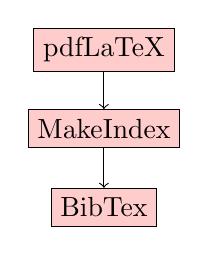
\begin{tikzpicture}
    \node (A) [rectangle, fill=red!20, draw] at (0, 0) {pdfLaTeX};
    \node (B) [rectangle, fill=red!20, draw] at (0, -1) {MakeIndex};
    \node (C) [rectangle, fill=red!20, draw] at (0, -2) {BibTex};
    \draw [->] (A) -- (B);
    \draw [->] (B) -- (C);
\end{tikzpicture}
\end{document}
